\chapter{Modelagem do Sistema Computacional}\label{sec:software}

O levantamento dos requisitos de um sistema é o elemento que fornece elementos que deve nortear uma série de decisões a serem tomadas no seu desenvolvimento. A ferramenta proposta visa agilizar o fluxo de trabalho do profissional que realiza análises de vida a fadiga, ou seja, propõem-se o seguinte fluxo padrão:

\begin{figure}[!ht]
    \centering
    \caption{Fluxo de operação proposto para a ferramenta.}\label{fig:workflow}
    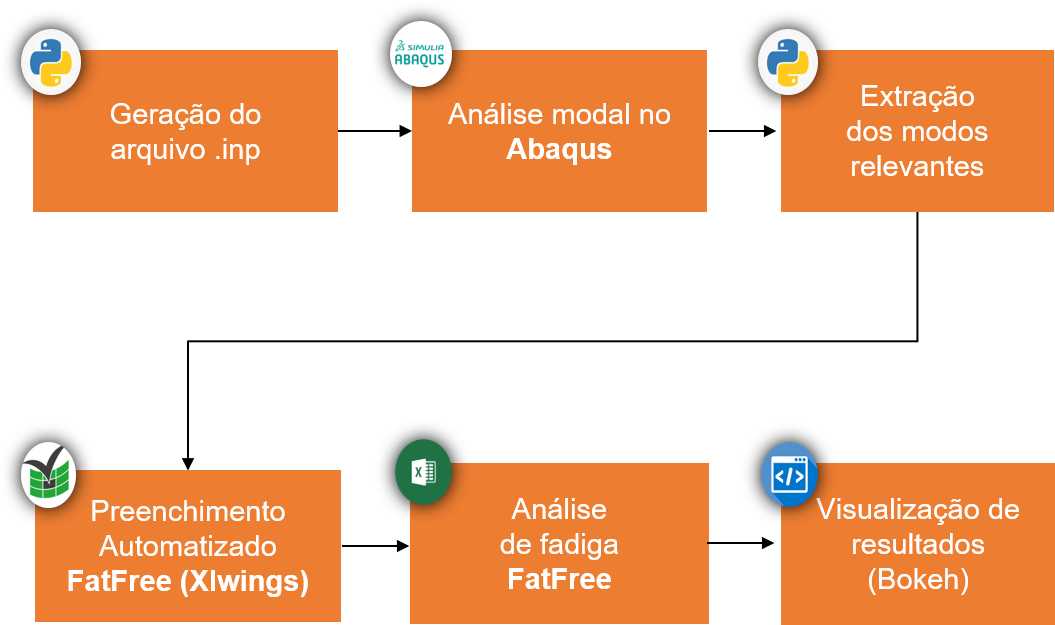
\includegraphics[width=0.7\textwidth]{imagens/workflow}
\end{figure}

De forma mais detalhada, a ferramente deve:

\begin{enumerate}
    \item A partir de um arquivo de entrada com informações do modelo, criar arquivos de entrada para o \abaqus (\texttt{.inp}) que reproduza todo o processo de simulação do comportamento do duto apresentado (\autoref{chap:assentamento}).
    \item Submeter o arquivo gerado para análise no \abaqus.\@
    \item Processar os arquivos de saída do \abaqus (\texttt{.odb}) extraindo os informações relevantes como a configuração deformada, modos de vibração, etc., gerando arquivos em outros formatos de fácil leitura para pós-processamento, tanto por esta ferramenta, quanto por outro \textit{softwares}.
    \item Pós-processar as informações gerando gráficos e relatórios relevantes para as tomadas de decisão do usuário quanto ao projeto. Esse é o requisito mais crítico, uma vez que é fundamental o entendimento sobre a análise de duto em vão livre. Entre as tarefas que fazem parte deste item está a automação da escolha dos modos de vibração ativos e relevantes e para cada vão de interesse -- a qual deve ser norteada pelos aspectos discutidos na~\autoref{sec:multimode} -- e a manipulação da FatFree\footnote{Planilha Microsoft Office Excel desenvolvida pela DNV-GL focada no cálculo de vida a fadiga de dutos submarinos.}.
    \item Apresentar os resultados finais na forma de gráficos e relatórios.
\end{enumerate}

\section{Linguagem de programação}

Python\footnote{https://www.python.org} foi a linguagem de programação adotada. Além de ser uma linguagem interpretada de alto nível Orientada a Objeto -- que permite um alto índice de reaproveitamento de código -- e da sintaxe simples, \citeonline{rao2018} apresenta algumas das principais vantagens que destaca a linguagem para este tipo de aplicação:

\begin{itemize}
    \item Disponibilidade de bibliotecas para aplicações cientificas contemplando manipulação de matrizes (Numpy), funções matemáticas (SciPy), manipulação de dados em forma tabular (Pandas), criação de gráficos interativos (Matplotlib e Bokeh).

    \item Suporte para automação de tarefas. Os recursos de \textit{script} internos do Python e vários pacotes têm um forte suporte à automação de tarefas. A automação de tarefas repetitivas e a realização do registro de dados são fáceis e requerem pouco esforço. O Abaqus, por exemplo, permite modelagem e acesso a informações em arquivos de saída via Python. A biblioteca xlwings permite manipulação planilhas Excel, a exemplo da FatFree.

    \item Pacotes Python como Django e Flask tornam possível desenvolver e usar o Python como uma API\footnote{Na programação de computadores, uma Interface de Programação de Aplicativos (\textit{Application Programming Interface} -- API) é um conjunto de definições de sub-rotinas e ferramentas para a criação de software. Em termos gerais, é um conjunto de métodos de comunicação claramente definidos entre vários componentes.} com um \textit{front-end} da web. Essa funcionalidade é particularmente útil para reaproveitamento da ferramenta em outras aplicações.
\end{itemize}

\subsection{Estrutura de módulos e classes}

Para implementação do fluxo de trabalho proposto para a ferramenta, prevê-se a implementações de módulos para lidar com cada contexto específico. São eles:

\begin{itemize}
    \item \texttt{model\_generator}: módulo principal responsável orquestrar o fluxo de trabalho da ferramenta desde o processamento dos dados de entrada, geração dos arquivos para o \abaqus e os pós-processamentos.

    \item \texttt{odb\_handler}: responsável por lidar com os arquivos de saída do \abaqus (odb) e guardar os dados relevantes em arquivos com formatos de fácil manipulação (CSV, JSON, etc\ldots).

    \item \texttt{mode\_selector}: módulo responsável pela estratégia de seleção automática de modos de vibração para cada vão e manipulação dos dados associados vãos e seus respectivos modos.

    \item \texttt{dnv}: módulo que implementa os cálculos do modelos de resposta da \dnvf105 e manipula a planilha FatFree por meio da biblioteca xlwings.

    \item \texttt{plots}: módulo responsável pro agregar as funções de geração de gráficos dos resultados.
\end{itemize}

Já dentre as principais classes estão:

\begin{itemize}
    \item \texttt{Model}: classe que contém as informações do modelo do problema.
    A classe armazena todas as informações para construção dos arquivos \texttt{.inp}, isto é, dados de batimetria, material, geometria do duto, coeficientes de segurança, entre outros.
    A instanciação dessa classe deve ocorrer mediante o processamento de um arquivo principal de entrada com esses dados, em formato JSON (\autoref{sec:estru_sim}).

    \item \texttt{Inp}: lida com a escrita modularizada de arquivos de entrada  para o \abaqus. A proposta é que se crie um arquivo principal que terá inclusão de outros arquivos acessórios que terão as informações específicas de cada aspecto da modelagem: batimetria, passos de carga, etc.

    \item \texttt{Span}: classe que representa um vão do duto. Dentre os métodos da classe estão os métodos responsáveis pela seleção dos modos de vibração.

    \item \texttt{ModeShape}: classe que representa um mode de vibração (\textit{mode shape}).
\end{itemize}

A \autoref{fig:UML} exibe um diagrama UML com esses módulos e classes, suas relações de pertencimento e dependência, e os principais métodos e atributos das classes.

\begin{figure}[!ht]
    \centering
    \caption{Diagrama UML dos módulos e classes.}\label{fig:UML}
    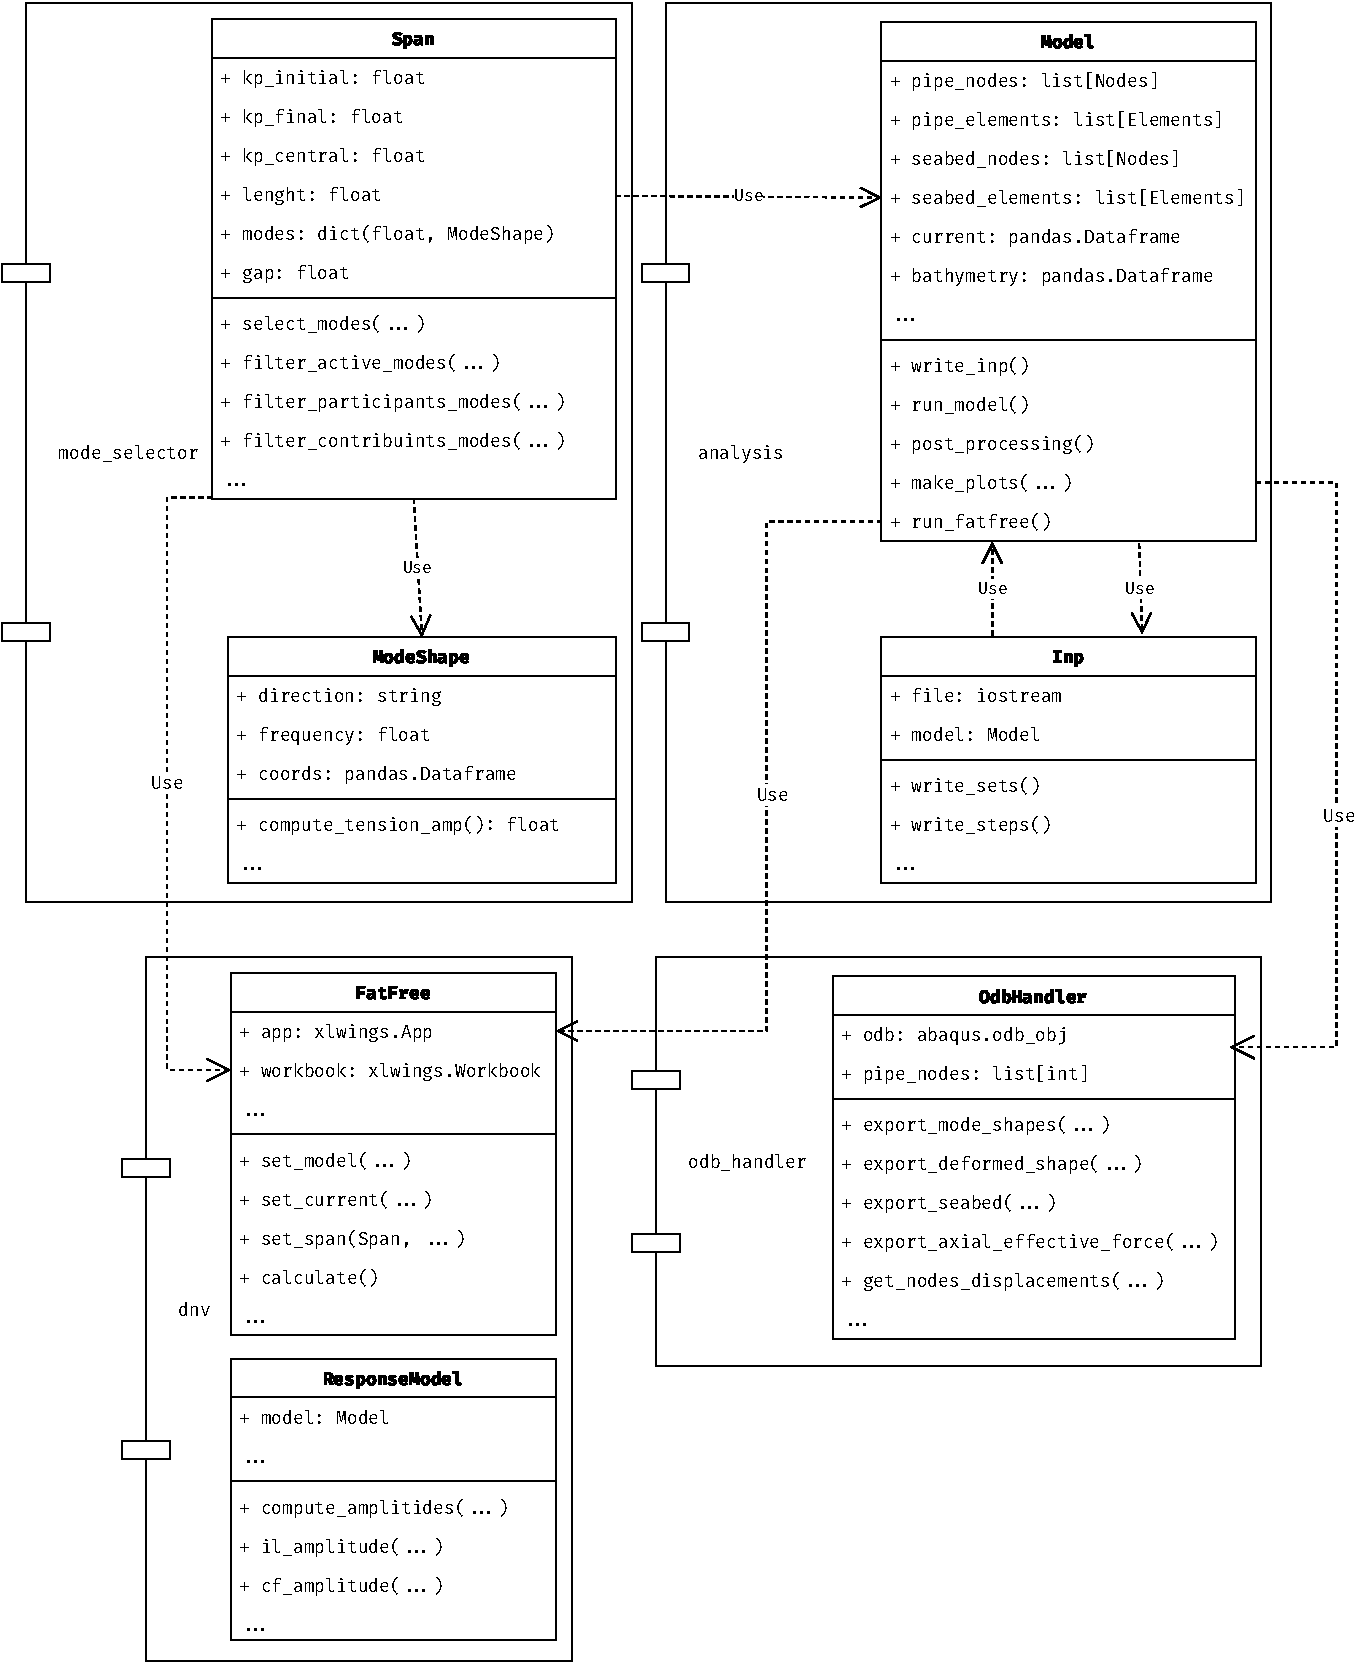
\includegraphics[width=0.95\textwidth]{imagens/UML}
    \fonte{Autor (2019)}
\end{figure}

\subsection{Arquivo de entrada (JSON)}\label{sec:estru_sim}

JSON é um formato de arquivo em texto puro que representa informações atribuindo um nome (ou rótulo) que descreve o seu significado e a seguir, o seu valor. Esta sintaxe de representação é derivada da forma utilizada pelo JavaScript para representar informações. Muito mais que um formato de arquivo, é um modelo para armazenamento e transmissão de informações no formato texto e que é bastante utilizado por aplicações \textit{Web}. A representação de informações utilizada em arquivos \texttt{json} é muito simples e sua forma de estruturação é bem mais compacta do que a que normalmente é feita em arquivos XML, o que torna o processamento das informações muito mais rápido.

A seguir descreve-se brevemente a estruturação do arquivo de entrada, apresentado nas listagens abaixo.
O arquivo foi feito pensando na facilidade do usuário em reconhecer os rótulos e preenchê-los de forma fácil e prática.
O arquivo compreende informações que servirão tanto para a análise do \abaqus (construindo um ou mais arquivos \texttt{.inp}) quanto para a \fatfree.

\begin{lstlisting}[language=json, label={tab:jdsn-arquivojson},caption={Exemplo de arquivo de entrada de dados - Parte 1/7}]
{
    "MODEL": {
        "NAME": "Duto_Piloto_X",
        "BATIMETRIA": "C:/Batimetria/batimetria.csv",
        "RESULTS_FOLDER": "C:/Resultados",
        "SPRING_PIPE_EXTREMITY": 0
    },
    "FILE_BAT": {
        "CPU": 12,
        "GPU": 12,
        "INTERACTIVE": 0
    },
    "CONDITIONS": {
        "TYPE_SEABED": 1,
        "CURTAIN_SPRINGS": 0,
        "RUN_MODEL": 1,
        "POST_PROCESSING": 1,
        "ISIGHT": 0,
        "SUPPORTS": true,
        "DELETE_FOLDER": false
    },
    "MODE_SELECTOR": {
        "NODESET": "PIPE",
        "ELEMENTSET": "PIPE",
        "SEABEDSET": "M_FUNDO",
        "SPANS": [
            {
                "kp_inicial": 9958.2,
                "kp_final": 9975.2,
                "azimute": 60.00
            }
        ],
        "N_MODES_IN_LINE": 4,
        "N_MODES_CROSS": 3
    },
    \dots
\end{lstlisting}

\begin{enumerate}
    \item \texttt{"MODEL"}: dados gerais do modelo, como:
    \begin{enumerate}
        \item \texttt{"NAME" (string)}: nome do arquivo;
        \item \texttt{"BATIMETRIA"  (string)}: indicação do arquivo de batimetria;
        \item \texttt{"RESULTS\_FOLDER"  (string)}: indicação do caminho para armazenamento dos resultados;
        \item \texttt{"SPRING\_PIPE\_EXTREMITY" (int)}: indicação da extremidade onde será colocada a mola, a mesma na qual foi aplicada a tração residual de lançamento.
    \end{enumerate}
    \item \texttt{"FILE\_BAT"}: para ser usado na performance da simulação.
    \begin{enumerate}
        \item \texttt{"CPU"}: número de núcleos disponíveis para simulação;
        \item \texttt{"GPU"}: número de núcleos da placa gráfica disponíveis para simulação;
        \item \texttt{"INTERACTIVE"}: garante que as simulações ocorram sequencialmente, e não simultaneamente.
    \end{enumerate}
    \item \texttt{"CONDITIONS"}: configurações gerais do modelo:
    \begin{enumerate}
        \item \texttt{"TYPE\_SEABED"}: \texttt{0} - Batimetria modelada com elementos do tipo R3D4. \texttt{1} - Batimetria modelada como superfície analítica,
        \item  \texttt{"CURTAIN\_SPRINGS}: \texttt{0} - A rigidez do solo é prescrita. \texttt{1} - A rigidez vertical é modelada como molas do tipo \textit{spring}.
        \item \texttt{"RUN\_MODEL"}: \texttt{0} - Utilizar o programa apenas para pós-processamento. \texttt{1} - rodar o modelo no \abaqus.
        \item \texttt{"POST\_PROCESSING"}: \texttt{0} - Rodar apenas a simulação no \abaqus. \texttt{1} - Após a simulação, iniciar diretamente o pós processamento.
        \item \texttt{"ISIGHT"}: chama diretamente o iSight caso seja necessário um processo de otimização ou DOE.
        \item \texttt{"SUPPORTS"}: \texttt{false} - não há suportes no modelo. \texttt{true} - indica que o modelo contém suportes.
        \item \texttt{"DELETE\_FOLDER"}: true - apaga a pasta de resultados e cria uma nova com os dados da nova simulação. \texttt{false} - não apaga a pasta de resultados.
    \end{enumerate}
    \item \texttt{"MODE\_SELECTOR"}: indica os dados necessários para o módulo de seleção de frequências.
    \begin{enumerate}
        \item \texttt{"NODESET"}: indica o \textit{nodeset} referente ao duto;
        \item \texttt{"ELEMENTSET"}: indica o \textit{elset} referente ao duto;
        \item \texttt{"SEABEDSET"}: indica o set referente à batimetria;
        \item \texttt{"SPANS"}: indica os vãos que serão submetidos ao pós-processamento.
        \item \texttt{"N\_MODES\_IN\_LINE"}: indica o número de nós que serão extraídos na direção \textit{in-line}.
        \item \texttt{"N\_MODES\_CROSS"}: indica o número de nós que serão extraídos na direção \textit{cross-flow}.
    \end{enumerate}
\end{enumerate}

\begin{lstlisting}[firstnumber=36, language=json, label={tab:jdsn-arquivojson2}, caption={Exemplo de arquivo de entrada de dados - Parte 2/7}]
    "ISIGHT": {
        "EXTRACTION_POINTS": [
            1431.8,
            1775.7
        ]
    },
    "PIPE_GEOMETRY": {
        "INITIAL_KP": 0,
        "END_KP": 1000,
        "LAUNCH_HEIGHT": -100,
        "LENGTH_ELEMENT": 0.25
    },
    "AUXILIARY_NODE": {
        "OFFSET_NODE_SPRING": 3,
        "INCREASE_FICTION_PLAN_X": 100,
        "INCREASE_FICTION_PLAN_Y": 10
    },
    "CURTAIN_SPRINGS": {
        "HEIGHT": -60,
        "STIFFNESS": [
            [
                -207904,
                -1
            ],
            [
                0,
                0
            ],
            [
                0,
                1
            ]
        ]
    },
\end{lstlisting}

\begin{enumerate}
    \item "ISIGHT": fornece os dados para pós-processamento no iSight.
        \begin{enumerate}
            \item \texttt{"EXTRACTION\_POINTS"}: indica os pontos que serão analisados no iSight.
        \end{enumerate}
    \item \texttt{"PIPE\_GEOMETRY"}: indica as informações relativas ao duto, como: comprimento, altura de lançamento e tamanho do elemento.
    \begin{enumerate}
        \item \texttt{"INITIAL\_KP"}: ponto de início do duto a ser modelado;
        \item \texttt{"END\_KP"}: ponto final do duto modelado;
        \item \texttt{"LAUNCH\_HEIGHT"}: altura de lançamento do duto, sob o qual será modelado a superfície fictícia;
        \item \texttt{"LENGHT\_ELEMENT"}: comprimento do elemento do tipo PIPE31 utilizado na modelagem do duto.
    \end{enumerate}
    \item \texttt{"AUXILIARY\_NODE"}: fornece os dados para a criação de nós auxiliares.
    \begin{enumerate}
        \item \texttt{"OFFSET\_NODE\_SPRING"}: define o \textit{offset} para a alocação da mola;
        \item \texttt{"INCREASE\_FICTION\_PLAN\_X"}: aumento lateral do plano fictício na extremidade inicial;
        \item \texttt{"INCREASE\_FICTION\_PLAN\_Y"}: aumento lateral do plano fictício na extremidade final;
    \end{enumerate}
    \item \texttt{"CURTAIN\_SPRINGS"}: caso o modelo seja simulado com cortina de molas, é necessário passar os dados para sua modelagem.
    \begin{enumerate}
        \item \texttt{"HEIGHT"}: cota vertical inicial das molas;
        \item \texttt{"STIFFNESS"}: dados de rigidez das molas.
    \end{enumerate}
\end{enumerate}


\begin{lstlisting}[firstnumber=70, language=json, label={tab:jdsn-arquivojson3}, caption={Exemplo de arquivo de entrada de dados - Parte 3/7}]
    "PIPE_MATERIAL": {
        "DENSITY": 9850.0,
        "ELASTICITY_MODULE": 2.07e11,
        "POISSON": 0.3,
        "COEFFICIENT_EXPANSION": 1.17e-5,
        "YIELD_STRESS": 4.15e8,
        "PLASTIC_DEFORMATION": 0.00,
        "EXTERNAL_RADIUS": 0.200,
        "THICKNESS": 0.0150
    },
    "SPRING_STIFFNESS": {
        "INITIAL": [
            [
                -1.0001e9,
                -10.0
            ],
            [
                1.0001e9,
                10.0
            ]
        ],
        "END": [
            [
                -1.0001e9,
                -10.0
            ],
            [
                1.0001e9,
                10.0
            ]
        ]
    },
\end{lstlisting}

\begin{enumerate}
    \item \texttt{"PIPE\_MATERIAL"}: fornece as propriedades do duto.
    \begin{enumerate}
        \item \texttt{"DENSITY"}: densidade;
        \item \texttt{"ELASTICY\_MODULE"}: módulo de elasticidade;
        \item \texttt{"POISSON"}: coeficiente de \textit{Poisson};
        \item \texttt{"COEFFICIENT\_EXPANSION"}: coeficiente de expansão térmica;
        \item \texttt{"YIELD\_STRESS"}: limite de escoamento do aço;
        \item \texttt{"PLASTIC\_DEFORMATION"}: limite de escoamento;
        \item \texttt{"EXTERNAL\_RADIUS"}: raio externo do duto;
        \item \texttt{"THICKNESS"}: espessura da parede duto.
    \end{enumerate}
    \item \texttt{"SPRING\_STIFFNESS"}: fornece os dados da rigidez das molas nas extremidades do duto.
    \begin{enumerate}
        \item \texttt{"INITIAL"}: dados da mola da extremidade inicial;
        \item \texttt{"END"}: dados da mola da extremidade final.
    \end{enumerate}
\end{enumerate}

\begin{lstlisting}[firstnumber=102, language=json, label={tab:jdsn-arquivojson4}, caption={Exemplo de arquivo de entrada de dados - Parte 4/7}]
    "CONTACT_PIPE_SEABED": {
        "HCRIT": 10000,
        "ELASTIC_SLIP": 0.001,
        "FRICTION_COEFF_1": 0.6,
        "FRICTION_COEFF_2": 0.8,
        "STABILIZE": 1e-8,
        "STIFFNESS": [
            [
                0,
                0
            ],
            [
                1000,
                1
            ]
        ]
    },
    "CONTACT_PIPE_PLAN": {
        "HCRIT": 10000,
        "ELASTIC_SLIP": 0.001,
        "EXTENSION_ZONE": 0.2,
        "FRICTION_COEFF_1": 0,
        "FRICTION_COEFF_2": 0.8,
        "STABILIZE": 1e-8,
        "STIFFNESS": [
            [
                0,
                0
            ],
            [
                1000,
                0.1
            ]
        ]
    },
\end{lstlisting}

\begin{enumerate}
    \item \texttt{"CONTACT\_PIPE\_SEABED"}: fornece as propriedades do contato entre o duto e a superfície referente à batimetria.
    \begin{enumerate}
        \item \texttt{"HCRIT"}: define quanto a superfície \textit{slave} pode penetrar na superfície \textit{master} antes que o \abaqus abandone o incremento atual e tente novamente com um incremento menor;
        \item \texttt{"ELASTIC\_SLIP"}: escoamento elástico permissível a ser usado no método de rigidez para aderência à fricção
        \item \texttt{"FRICTION\_COEFF\_1"}: coeficiente de atrito;
        \item \texttt{"FRICTION\_COEFF\_2"}: coeficiente de atrito;
        \item \texttt{"STABILIZE"}: parâmetro de estabilidade do contato;
        \item \texttt{"STIFFNESS"}: dados de rigidez do solo, para interação duto-solo.
    \end{enumerate}
    \item \texttt{"CONTACT\_PIPE\_PLAN"}: fornece as propriedades do contato entre o duto e a superfície fictícia.
\end{enumerate}


\begin{lstlisting}[firstnumber=137, language=json, label={tab:jdsn-arquivojson5}, caption={Exemplo de arquivo de entrada de dados - Parte 5/7}]
    "STEPS_DEFAULTS": {
        "MAXIMUM_INCREMENT_NUMBER": 10000,
        "AUTOMATIC_STABILIZATION": 1.0e-8,
        "INITIAL_SIZE_INCREMENT": 0.0001,
        "TOTAL_STEP_TIME": 0.01,
        "MINIMUM_INCREMENT_SIZE": 1.0e-30,
        "MAXIMUM_INCREMENT_SIZE": 0.01
    },
    "STEP_1": {
        "EMPTY_SUBMERSE_WEIGHT": 1.4
    },
    "STEP_2": {
        "INITIAL_SIZE_INCREMENT": 0.1,
        "TOTAL_STEP_TIME": 2.1,
        "MAXIMUM_INCREMENT_SIZE": 2.1,
        "EXTERNAL_PRESSURE": 103542.25,
        "EFFECTIVE_DIAMETER": 0.4523
    },
    "STEP_3": {
        "INITIAL_SIZE_INCREMENT": 0.001,
        "RELEASE_TRACTION": 35000.00
    },
    "STEP_4": {
        "MAXIMUM_INCREMENT_NUMBER": 100000,
        "DISPLACEMENT_FICTITIOUS_PLANE": -200.00
    },
    "STEP_5": {},
    "STEP_6": {},
    "STEP_7": {},
    "STEP_8": {
        "INITIAL_SIZE_INCREMENT": 0.1,
        "TOTAL_STEP_TIME": 24.93,
        "MAXIMUM_INCREMENT_SIZE": 5.00,
        "INTERNAL_PRESSURE": 3654453.0,
        "WEIGHT_SUBMERGED_FLOODED": 2.62
    },
\end{lstlisting}

\begin{enumerate}
    \item \texttt{"STEPS\_DEFAULTS"}: reúne as informações recorrentes em todos os \textit{steps} no arquivo \texttt{*.inp}.
    \begin{enumerate}
        \item \texttt{"MAXIMUM\_INCREMENT\_NUMBER"}: define o máximo de incrementos para o \textit{step};
        \item \texttt{"AUTOMATIC\_STABILIZATION"}: parâmetro de estabilização para casos onde há contato;
        \item \texttt{"INITIAL\_SIZE\_INCREMENT"}: valor inicial do incremento;
        \item \texttt{"TOTAL\_STEP\_TIME"}: tempo total no \textit{step};
        \item \texttt{"MINIMUM\_INCREMENT\_SIZE"}: número mínimo de incrementos para o \textit{step};
        \item \texttt{"MAXIMUM\_INCREMENT\_SIZE"}: número máximo de incrementos para o \textit{step}.
    \end{enumerate}
    \item \texttt{"STEP\_X"}: informação específica para cada \textit{step} conforme os passos de carga anteriormente citados. Caso existam informações específicas do suporte, essas informações devem ser passadas respectivamente. Caso contrário, são utilizadas as informações do \texttt{"STEP\_DEFAULTS"}.
\end{enumerate}

\begin{lstlisting}[firstnumber=173, language=json, label={tab:jdsn-arquivojson6}, caption={Exemplo de arquivo de entrada de dados - Parte 6/7}]
    "STEP_9": {
        "INITIAL_SIZE_INCREMENT": 0.1,
        "TOTAL_STEP_TIME": 24.93,
        "MAXIMUM_INCREMENT_SIZE": 5
    },
    "STEP_10": {
        "INITIAL_SIZE_INCREMENT": 0.1,
        "TOTAL_STEP_TIME": 15.12,
        "MAXIMUM_INCREMENT_SIZE": 5,
        "WEIGHT_SUBMERGED_OPERATIONAL": 0.85,
        "OPERATION_PRESSURE": 1265413
    },
    "STEP_11": {
        "NUMBER_MODES": 100,
        "MAXIMUM_NUMBER_INTERACTIONS": 200
    },
    "SUPPORTS": {
        "FILE_DEFORMED_IN_LOCO": "D:/Batimetria/arquivo_survey.eff",
        "SHIFT_SURFACE": 10,
        "STEP": 7,
        "LIST": [
            [
                [
                    845,
                    1
                ]
            ],
            [],
            [],
            []
        ]
    },
    "STEP_NODAL_FIX": {},
    "STEP_SURFACE_SUPPORTS": {},
\end{lstlisting}

\begin{enumerate}
    \item \texttt{"SUPPORTS"}: reúne as informações referentes à posição dos suportes.
    \begin{enumerate}
        \item \texttt{"FILE\_DEFORMED\_IN\_LOCO"}: caminho para o arquivo de \textit{topping}. O arquivo é utilizado como base de comparação para alocação dos suportes;
        \item \texttt{"SHIFT\_SURFACE"}: %%%%%%%% ;
        \item \texttt{"STEP"}: \textit{step} a partir do qual serão alocados os suportes;
        \item \texttt{"LIST"}: lista de suportes de acordo com o tipo implementado. São passados o KP centro do suporte e o comprimento do mesmo.
        \begin{enumerate}
            \item No primeiro conjunto de colchetes são passados suportes do tipo \textit{grout bag}, posicionados abaixo do duto;
            \item Em seguida, suportes do tipo manta, posicionados acima do duto;
            \item No terceiro colchete, suportes mecânicos do tipo pino (restrição de deslocamentos transversais ao eixo do duto e as rotações nodais).
            \item Por fim, suportes mecânicos do tipo livre (restrição de deslocamento transversal ao eixo do duto)
        \end{enumerate}
    \end{enumerate}
    \item \texttt{"STEP\_NODAL\_FIX"}: \textit{Step} no qual serão aplicadas as restrições nodais, relacionadas aos diferentes tipos de suporte. Chave vazia refere-se aos valores passados na \textit{keyword} \texttt{STEPS\_DEFAULTS}.
    \item \texttt{"STEP\_SURFACE\_SUPPORTS"}: \textit{Step} no qual a superfície analítica referentes aos suportes são posicionadas. Chave vazia refere-se aos valores passados na \textit{keyword} \texttt{STEPS\_DEFAULTS}.
\end{enumerate}

\begin{lstlisting}[firstnumber=207, language=json, label={tab:jdsn-arquivojson7}, caption={Exemplo de arquivo de entrada de dados - Parte 7/7}]
    "FATFREE": {
        "CURRENT_FILE": "D:/Corrente/arquivo_de_corrente.csv",
        "ISIGHT_FILE": "D:/Resultados/DutoX_trecho3/isight.txt",
        "h": 165,
        "L": 70,
        "e": 0.88,
        "d": 0,
        "teta_pipe": 0,
        "z_structure": 0.005,
        "z_soil_in_line": 0.02,
        "z_soil_cross_flow": 0.014,
        "z_hRM": 0,
        "Kv": 1.33e7,
        "KL": 1e7,
        "Kv_s": 2.5e5,
        "SCF": 1,
        "kc": 0,
        "fcn": 42,
        "k": 0.0033,
        "p": 124.54,
        "DT": 0.02062,
        "Ds": 0.3238,
        "t_concrete": 0,
        "t_coating": 0.003,
        "r_steel": 7850,
        "r_concrete": 0,
        "r_coating": 935,
        "r_cont": 200,
        "Turbulence_intensity_Ic": 0.04,
        "Measurement_ref_Height_zr": 5,
        "On_bottom_roughness_z0": 0.00004,
        "Time_between_independent_current_events": 1.0,
        "Flag": false
    }
}
\end{lstlisting}

\begin{enumerate}
    \item \texttt{"FATFREE"}: passa os dados necessários para preenchimento da \fatfree via \textit{xlwings}.
    \begin{enumerate}
        \item \texttt{"CURRENT\_FILE"}: indica caminho para o arquivo de corrente, retirado das ETs forncecidas pela na forma de histograma. A rotina realiza os cálculos necessários para incluir os dados na \textit{sheet Current} da planilha de cálculo;
        \item \texttt{"ISIGHT\_FILE"}: indica o caminho onde será salvo o arquivo \texttt{*.txt} com os dados que serão utilizados para o pós-processamento no iSight;
        \item \texttt{"Flag"}: permite o usuário escolher se os dados de rigidez (Kv, KL e  Kv\_s) serão os passados pelo usuário acima ou extraídos do \abaqus.
    \end{enumerate}
\end{enumerate}
